%%%%%%%%%%%%%%%%%%%%%%%%%%%%%%%%%%%%%%%%%%%%%%%%%%%%%%%%%%%%%%%%%%%%%%%%%%%%%%%%%%%%%%%%%%
%%
%% Description:		This is an example presentation using the beamerthemedhbw
%%
%%					The beamerthemedhbw is based on jacksbeamertheme
%%					(https://github.com/JacknJo/jacksbeamertheme)
%%
%% Author:			Hannes Bartle																				
%% 					DHBW Ravensburg Campus Friedrichshafen		
%%					September 2016	
%% 
%% The beamerthemedhbw is free software: you can redistribute it and/or modify
%% it under the terms of the GNU General Public License as published by
%% the Free Software Foundation, either version 3 of the License, or
%% (at your option) any later version.
%% 
%% The beamerthemedhbw is distributed in the hope that it will be useful,
%% but WITHOUT ANY WARRANTY; without even the implied warranty of
%% MERCHANTABILITY or FITNESS FOR A PARTICULAR PURPOSE.  See the
%% GNU General Public License for more details.
%% 
%% You should have received a copy of the GNU General Public License
%% along with the beamerthemedhbw.  If not, see <http://www.gnu.org/licenses/>.
%% 
%% 
%%%%%%%%%%%%%%%%%%%%%%%%%%%%%%%%%%%%%%%%%%%%%%%%%%%%%%%%%%%%%%%%%%%%%%%%%%%%%%%%%%%%%%%%%%


\documentclass[	12pt, 				
				t,					
				aspectratio=169,
				%handout-PLACEHOLDER
				]{beamer}

\usepackage{dhbwstyle}

\title{Ergänzungen zu Datentypen\&Wildcards}

\begin{document}
	
	\begin{frame}[noframenumbering]
		\titlepage
	\end{frame}


	\begin{frame}{Outline}
		\tableofcontents
	\end{frame}
    
    \outlineFrame{Mehrfachvererbung vs. Interfaces}
    
    \begin{frame}{Mehrfachvererbung oder Interfaces?}{Was ist besser?}
\textbf{Was kann Mehrfachvererbung, das Interfaces nicht können?}
    \begin{itemize}[<+->]
        \item Kurzgesagt: Funktional lässt sich beides äquivalent nutzen
        \item Der Unterschied liegt vielmehr in formaler Betrachtung der OOP
        \item Mehrfachvererbung birgt aber viele Risiken
        \begin{itemize}
            \item Diamond-Problem
            \item Komplexe (=undurchsichtige) Vererbungshierarchien
            \item Falsche Verwendung
        \end{itemize}
    \end{itemize}
\end{frame}

\begin{frame}{Diamond-Problem}{Visuelle Darstellung}
    \begin{figure}
        \centering
        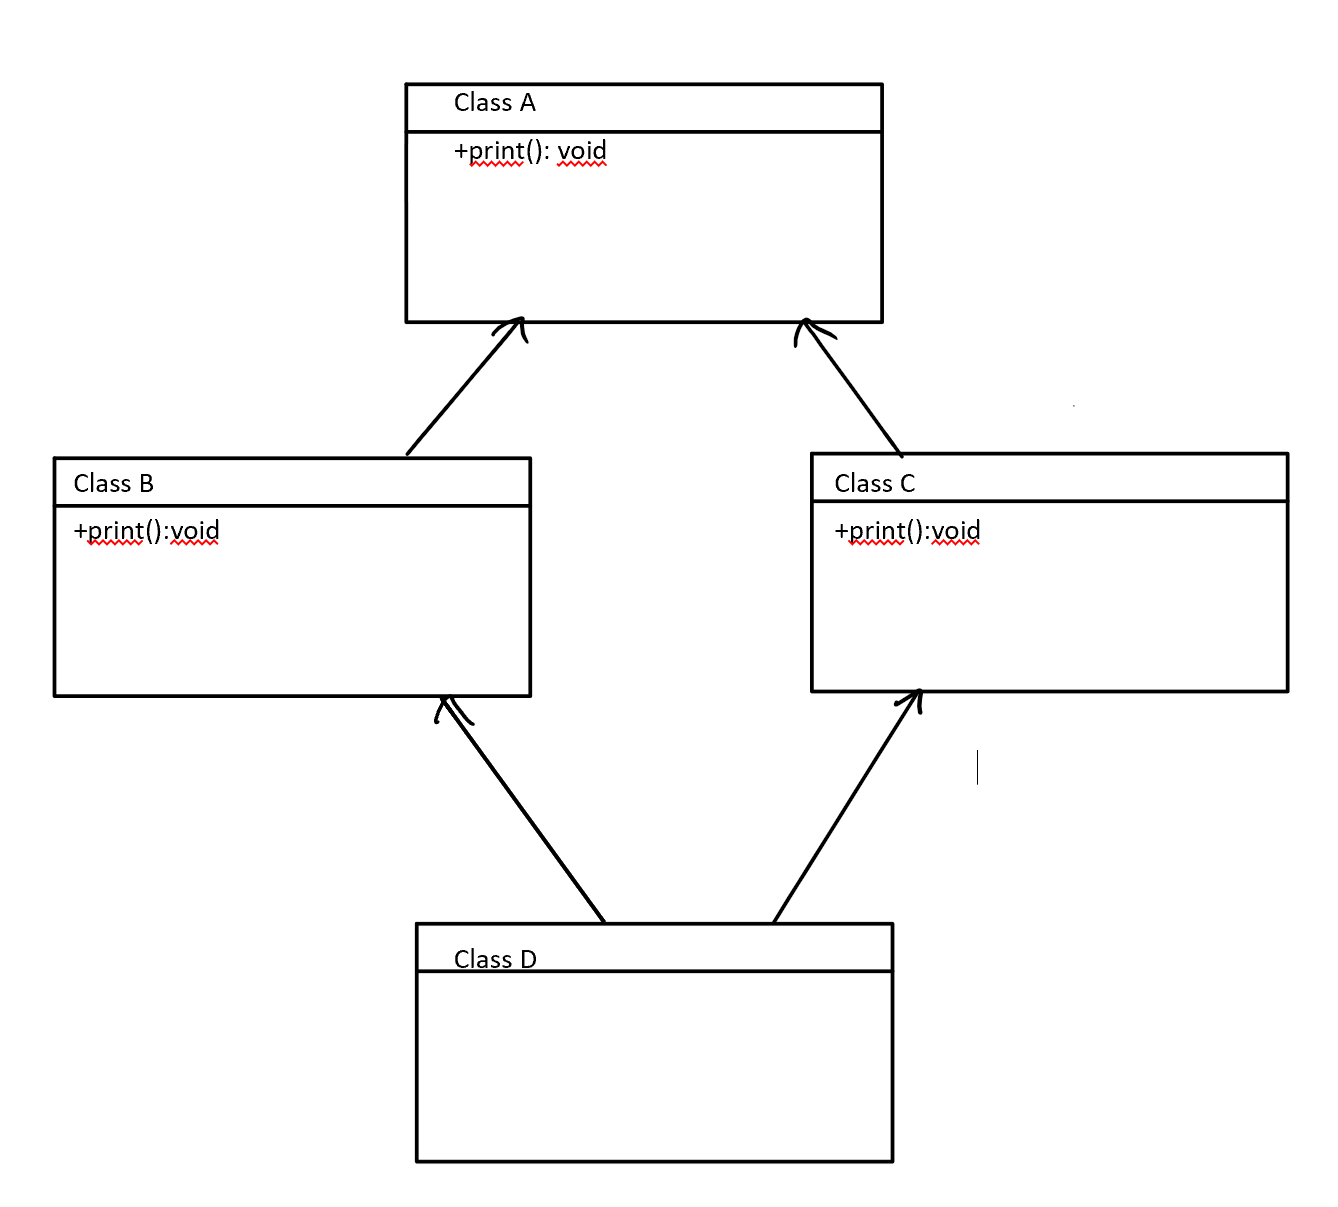
\includegraphics[height=4.5cm]{graph/diamond}
    \end{figure}
\end{frame}

\begin{frame}{Diamond-Problem}{Kurze Erklärung}
    \begin{itemize}
        \item Tritt auf, wenn die "`Großvaterklasse"' von zwei Basisklassen gleich ist
        \item Führt zu einer Mehrdeutigkeit in Methoden und Member Variablen
        \item Diese wird jedoch in den meisten Sprachen durch den Compiler abgefangen
        \item Diamond Problem \textit{kann} auch in Java auftreten
        \begin{itemize}
            \item Weil Default-Implementierungen von Interfaces erlaubt sind
            \item Werden auch durch Compiler erkannt
            \item Entwickler \textbf{muss} Klassenspezifische Implementierung erstellen
        \end{itemize}
    \end{itemize}
\end{frame}

\begin{frame}[fragile]{Diamond-Problem}{Am Java Beispiel}
\lstset{style=java}
\begin{lstlisting}
public interface A{
    public void say(){
        print("I am A!");
    }
}

public interface B{
    public void say(){
        print("I am B");
    }
}

public class C implements A,B{
    //Compilerfehler, weil say() mehrdeutig ist!
}
\end{lstlisting}
\end{frame}

\begin{frame}{Das Problem der Mehrfachvererbung}
    \begin{itemize}
        \item Oft falsch verwendet
        \item Besonders bei Anfängern
        \item Wo keine Mehrfachvererbung ist, kann sie nicht falsch verwendet werden $\Rightarrow$ Der Java Ansatz
        \item Statt Mehrfachvererbung hilft oft:
        \begin{itemize}
            \item Assoziation
            \item Aggregation
            \item Komposition
            \item Delegation
        \end{itemize}
    \end{itemize}
\end{frame}

\begin{frame}{Assoziation}
\begin{itemize}
    \item Beziehung zwischen zwei Objekten
    \item Es besteht jedoch keine Abhängigkeit
    \item Beide Objekte können unabhängig voneinander existieren
    \item Beispiel: Relation zwischen Sprecher und Zuhörer
\end{itemize}
\begin{figure}
    \centering
    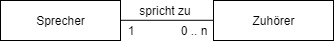
\includegraphics[width=0.8\textwidth]{graph/association}
\end{figure}
\end{frame}

\begin{frame}{Aggregation}
\begin{itemize}
    \item Sonderfall der Assoziation
    \item Hier eine unidirektionale Beziehung (\textbf{"`benötigt ein"'} Beziehung)
    \item Kindobjekt kann unabhängig von Elternobjekt existieren
    \item Aber Elternobjekt nicht ohne Kind
    \item Beispiel: Auto und Räder
    \begin{itemize}
        \item Räder können auch ohne Auto sinnvoll sein
        \item Autos ohne Räder eher weniger...
    \end{itemize}
\end{itemize}
\begin{figure}
    \centering
    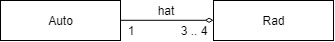
\includegraphics[width=0.8\textwidth]{graph/aggregation}
\end{figure}
\end{frame}

\begin{frame}{Komposition}
    \begin{itemize}
        \item Sonderfall der Aggregation
        \item Strenge Abhängigkeit zwischen kind- und Elternobjekt
        \item Beide können nicht unabhängig voneinander existieren
        \item Beispiel: Mensch und Herz
    \end{itemize}
\begin{figure}
    \centering
    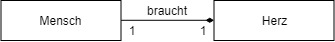
\includegraphics[width=0.8\textwidth]{graph/composition}
\end{figure}
\end{frame}

\begin{frame}{Delegation}
    \begin{itemize}
        \item Ist ein alternativer Ansatz zur Vererbungshierarchien
        \item Hierbei wird ein Objekt als Instanzvariable genutzt
        \item Funktionsaufrufe werden "`durchgereicht"' an dieses
        \item Vorteil gegenüber Vererbung/Interfaces:
        \begin{itemize}
            \item Nicht alle Methoden müssen nach außen sichtbar gemacht werden
            \item Für Delegate kann spezielle Unterklasse genutzt werden
        \end{itemize}
    \end{itemize}
\end{frame}

\begin{frame}[fragile]{Delegation}{Codebeispiel}
\lstset{style=java}
\begin{lstlisting}
public class Delegate(
    public void print(){
        System.out.println("I am a Delegate!");
    }    
    public void sayHello(){
        System.out.println("Hello!");
    }
)

public Class Example{
    private Delegate del = new Delegate();
    
    public void print(){
        del.print();
    }
}
\end{lstlisting}
\end{frame}

\begin{frame}{Schlechte Mehrfachvererbung}
    \begin{itemize}
        \item Wir haben eine Klasse \texttt{Rad} und \texttt{Motor}
        \item Man möchte nun eine \texttt{Auto} Klasse implementieren
        \item Ein unerfahrener Nutzer denkt:
        \begin{itemize}
            \item Ein Auto braucht Fähigkeiten vom \texttt{Rad}
            \item ...und vom \texttt{Motor}
            \item und entwirft folgende Klasse:
        \end{itemize}
    \end{itemize}
\end{frame}

\begin{frame}{Schlechte Mehrfachvererbung}{Am Beispiel}
    \begin{figure}
        \centering
        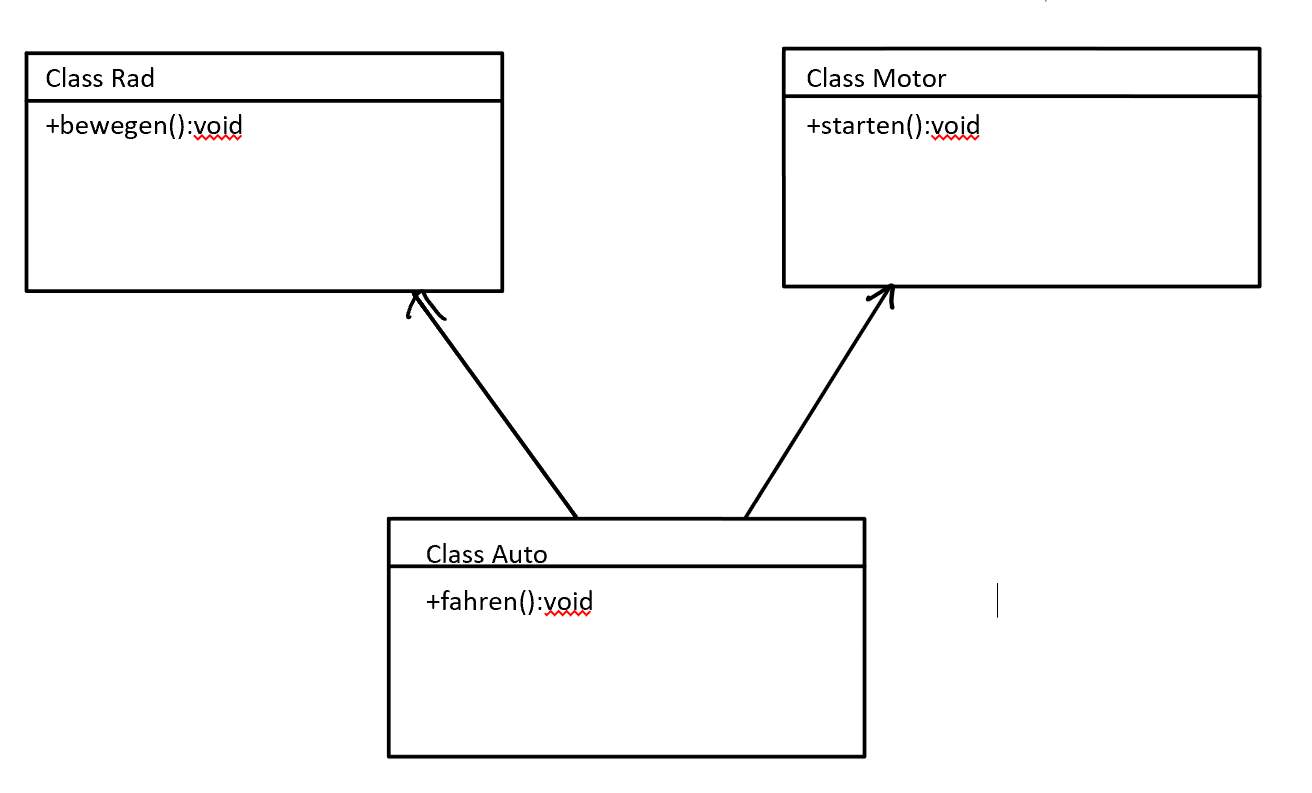
\includegraphics[height=4.5cm]{graph/badMI}
    \end{figure}
\end{frame}

\begin{frame}{Gute Verwendung von Mehrfachvererbung}
\begin{itemize}
    \item Sind relativ selten
    \item Wenige reale Anwendungsfälle
    \item Ein Beispiel: "`Mix-in Klassen"'
    \begin{itemize}
        \item Nutzt im Grunde Mehrfache Verkettung von Template Klassen (Generics)
        \item Link für mehr Info(C++): \href{http://www.thinkbottomup.com.au/site/blog/C\%20\%20_Mixins_-_Reuse_through_inheritance_is_good}{Mix-in} (Siehe \cite{mixin})
    \end{itemize}
\end{itemize}
\end{frame}

\begin{frame}{Der Zusammenhang zu Interfaces}
    \begin{itemize}[<+->]
        \item Laut formalen OOP:
        \begin{itemize}
            \item Definiert \textit{Vererbung} eine \textbf{"`ist ein"'} Beziehung
            \item Und ein \textit{Interface} eine \textbf{"`Hat die Fähigkeit"'} Beziehung
        \end{itemize}
        \item Heißt, formal "`darf"' man ein Interface nicht als Mehrfachvererbung betrachtet werden
        \item ...ist aber irgendwie nicht weit davon weg
        \item Verstößt Java damit gegen die Prinzipien der OOP?
        \begin{itemize}[<handout:0>]
            \item Ganz klares: "`Jain"'
            \item Kaum eine Sprache erfüllt alle Anforderungen an OOP
        \end{itemize}
    \end{itemize}
\end{frame}

\begin{frame}{"`Richtige"' Eigenschaften von Interfaces}
    \begin{itemize}
        \item Rein abstrakte Definition von Schnittstellen
        \item Keine Attribute
        \item Keine Assoziationen
        \item Definiert eine Menge von Operationen $\Rightarrow$ Eigentlich ohne Implementierung
    \end{itemize}
\end{frame}

    
    \outlineFrame{Wildcards}
    
    \begin{frame}{Generics}{...und die Vererbung nochmal}
    \begin{itemize}
        \item Hauptgrund für Wildcards: Die "`eigenartige"' Vererbung bei generischen Klassen:
        \begin{itemize}
            \item Wenn \texttt{Integer} von \texttt{Number} erbt...
            \item Warum dann nicht auch \texttt{List<Integer>} von \texttt{List<Number>}?
        \end{itemize}
        \item Würde dazu führen, dass man inkompatible Typen zuweisen kann
        \begin{itemize}
            \item Zum Beispiel einen Double in eine \texttt{List<Integer>}
        \end{itemize}
    \end{itemize}
\end{frame}

\begin{frame}[fragile]{Generic-Vererbung}{Ein Gegenbeispiel}
\lstset{style=java}
\begin{lstlisting}
List<Number> ln = new List<Number>();
List<Integer> li = {7,12,42,46};
ln = li;    //li wird als Referenz übergeben!
//Hier würde man li einen Double hinzufügen:
ln.add(new Double(2.7182818284590));
\end{lstlisting}
\end{frame}

\begin{frame}{Wildcards}{Und deshalb braucht man sie}
    \begin{itemize}
        \item Durch "`ungewöhnliche"' Vererbungshierarchie von Generics benötigt
        \item Definieren einen unbekannten Typ
        \begin{itemize}
            \item Der jedoch eingeschränkt werden kann
            \item ...Wie bereits letztes mal besprochen
        \end{itemize}
        \item Verwendung als Argument von Funktionen
        \item Oder auch als Rückgabewert (Eher vermeiden)
    \end{itemize}
\end{frame}

\begin{frame}[fragile]{Wildcards}{Verwendung}
\lstset{style=java}
\begin{lstlisting}
void someFunc(List<?> in){ /* ... */ }   //OK
List<?> func(){ /* ... */ }              //OK

List<?> l1;   //OK
List<?> l2 = new ArrayList<>();   //OK
List<?> l3 = new ArrayList<?>();  //Fehler
\end{lstlisting}
\end{frame}

\begin{frame}{Upper-Bounded Wildcards}{Hoffentlich etwas klarer}
    \begin{itemize}[<+->]
        \item Einschränkung des Generics nach oben
        \item Dadurch gemeinsame Funktionalitäten, egal was übergeben wird
        \item \texttt{<?>} ist formal gesehen ein \texttt{<? extends Object>}
        \item Können jedoch nur lesend verwendet werden
        \item Warum?
        \begin{itemize}[<handout:0>]
            \item Beispiel \texttt{add(T)} auf eine \texttt{List<? extends Number>}
            \item Es gibt keinen Typ \texttt{T}, der auf alle Varianten von \texttt{<? extends Number>} passt
            \item Kurz: Wir können nicht sicherstellen, ob der Typ den wir schreiben überhaupt mit der speziellen Instanz kompatibel ist!
            \item Einzige Ausnahme: \texttt{null}
        \end{itemize}
    \end{itemize}
\end{frame}

\begin{frame}{Upper-Bounded Wildcards}{Visualisiert}
    \begin{figure}
        \centering
        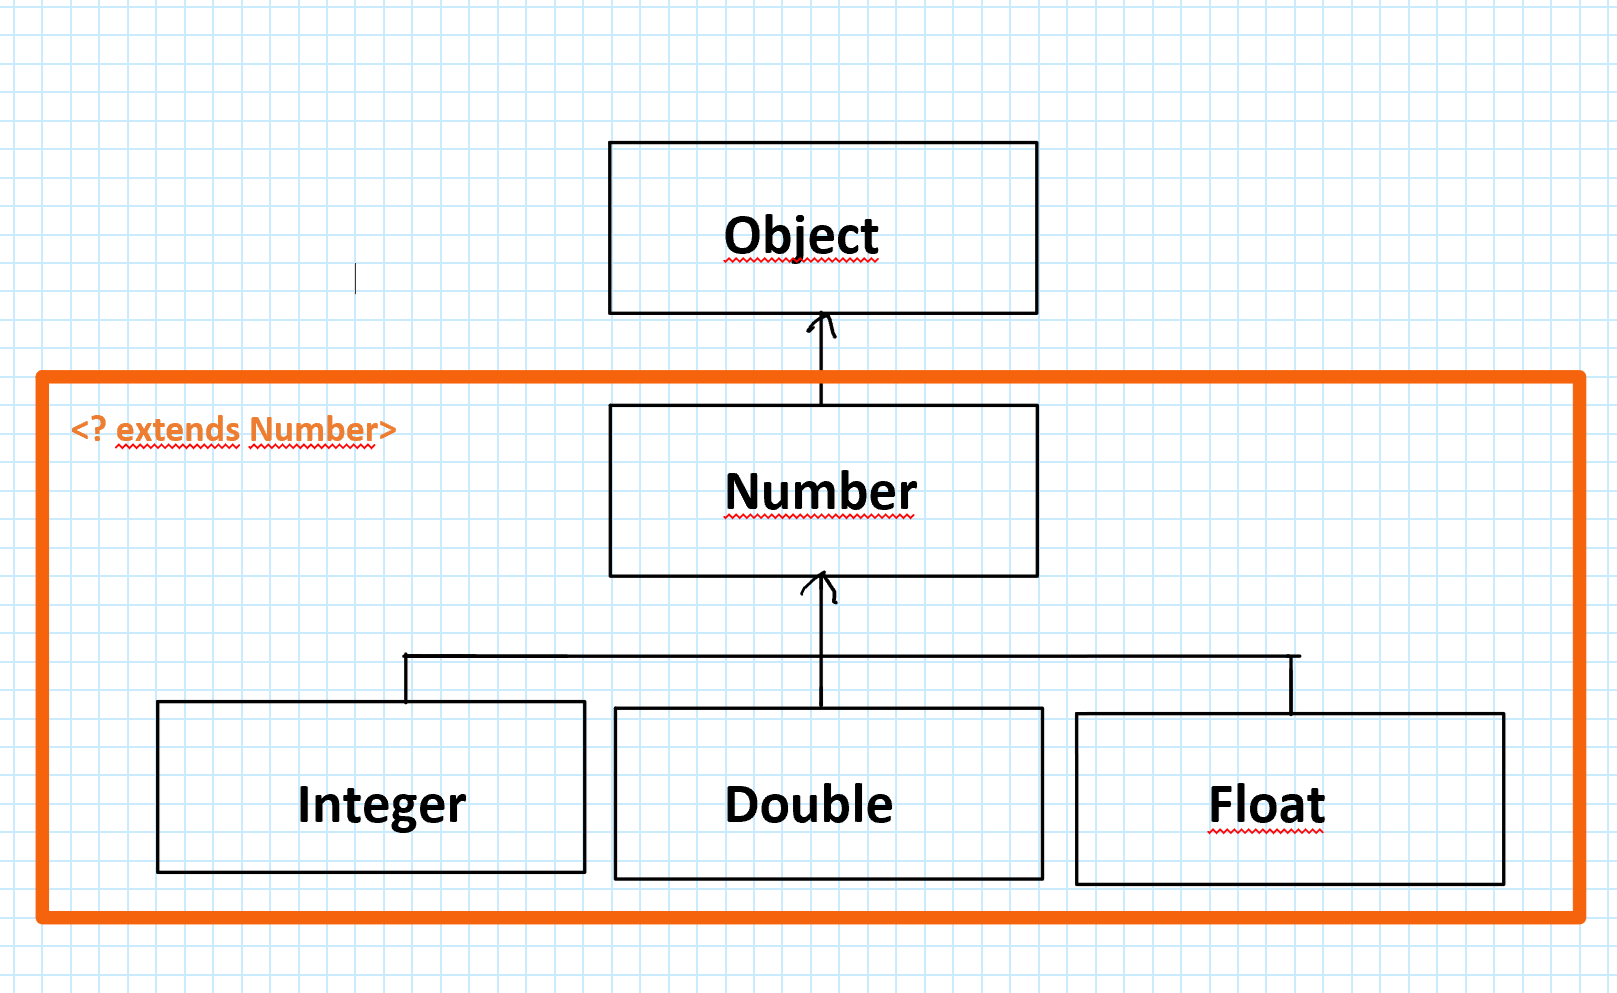
\includegraphics[height=4.5cm]{graph/wildcard_upper}
    \end{figure}
\end{frame}

\begin{frame}{Lower-Bounded Wildcards}{Nochmal erklärt}
    \begin{itemize}[<+->]
        \item Beschränken die Klasse nach unten
        \item Umgekehrter Effekt zu Upper-Bound Wildcards:
        \begin{itemize}
            \item Wir keinen lesenden Zugriff (Außer über Methoden von \texttt{Object})
            \item Dafür aber schreibeneden
            \item Dadurch keine gemeinsamen Schnittstellen
            \item Aber gemeinsamer Typ, der auf alle möglichen übergebenen Klassen passt
        \end{itemize}
        \item Frage: Welches ist dieser gemeinsame Typ? (Zum Beispiel für \texttt{List<? super Number>)}
        \begin{itemize}[<handout:0>]
            \item Immer "`unterste"' Typ (Im Sinne der Vererbung)
            \item Durch die \textbf{"`ist ein"'} Beziehung passt dieser auf alle anderen Klassen
        \end{itemize}
    \end{itemize}
\end{frame}

\begin{frame}{Lower-Bounded Wildcards}{Visualisiert}
    \begin{figure}
        \centering
        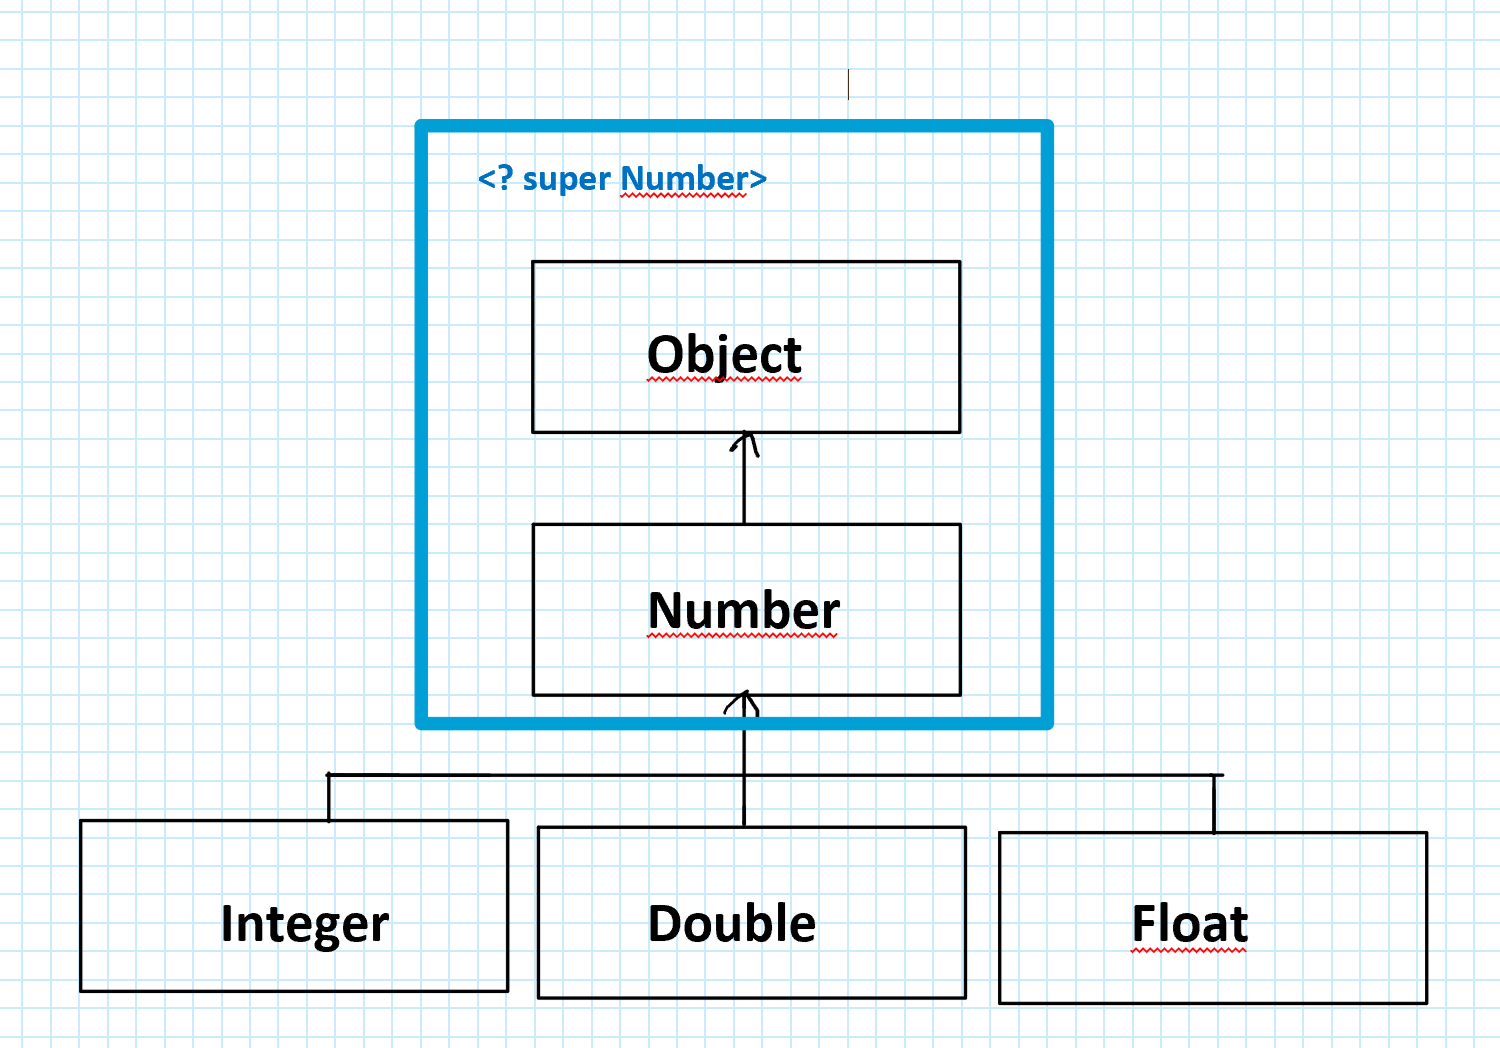
\includegraphics[height=4.5cm]{graph/lower_wildcard}
    \end{figure}
\end{frame}

\begin{frame}{Bounded Wildcards}{Nochmal in der Übersicht}
    \begin{figure}
        \centering
        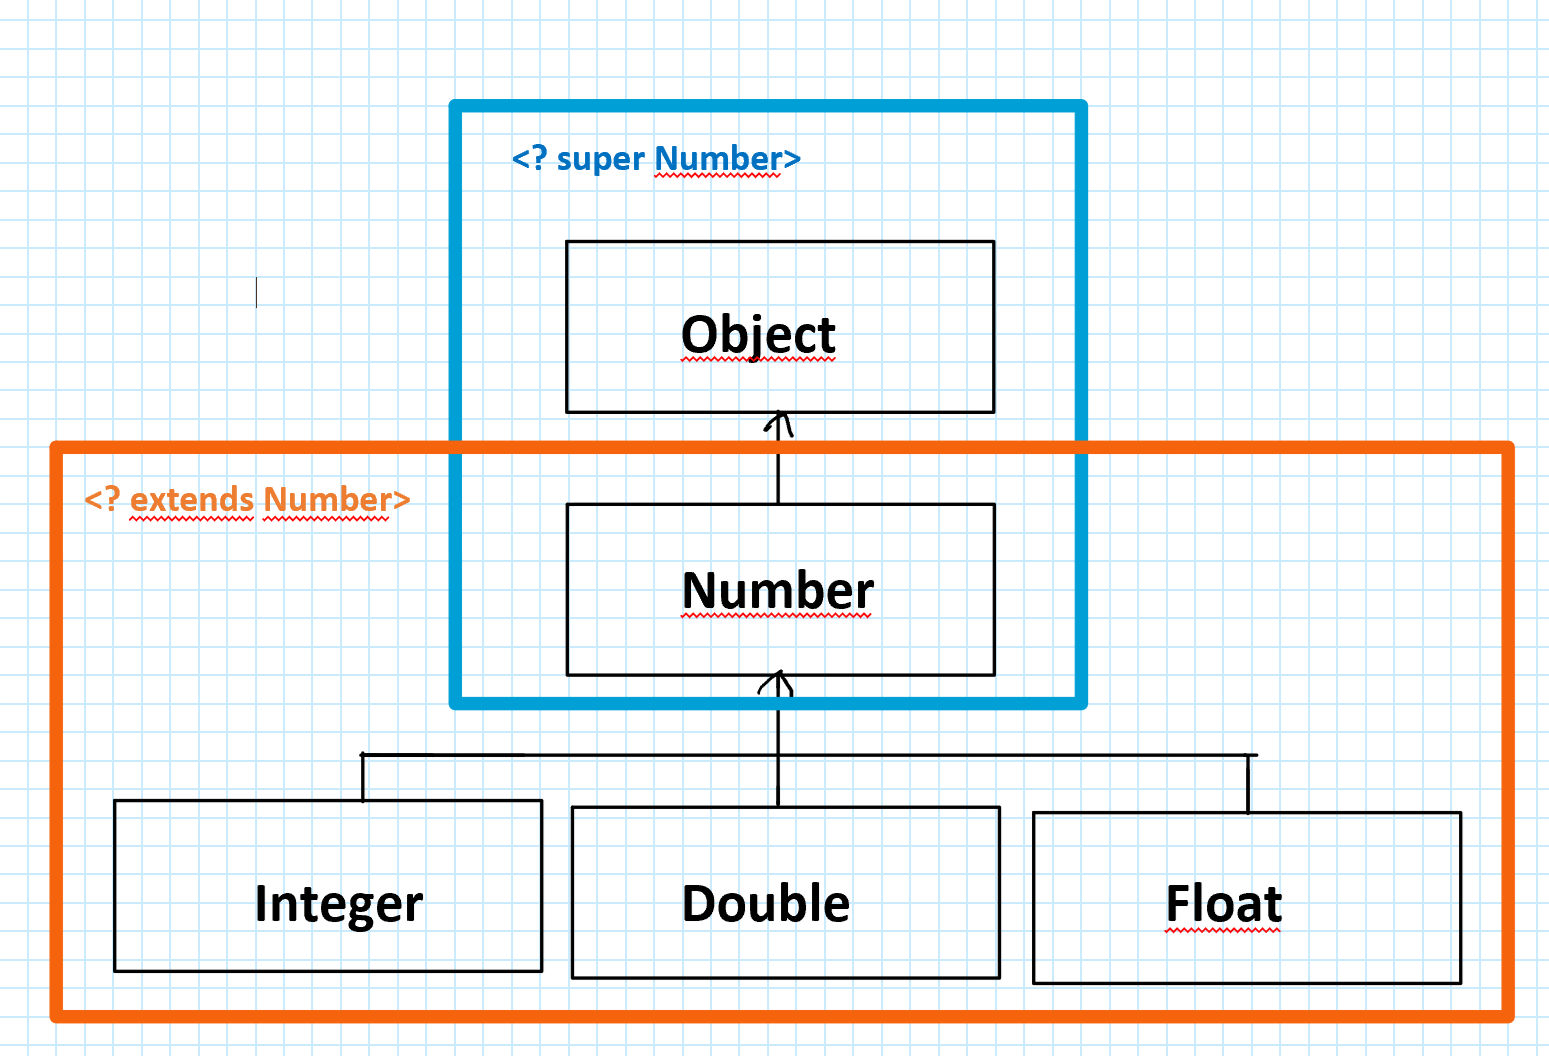
\includegraphics[height=4.5cm]{graph/wildcard_bound}
    \end{figure}
\end{frame}

\begin{frame}{Wildcards}{Und deren Vererbung}
    \begin{figure}
        \centering
        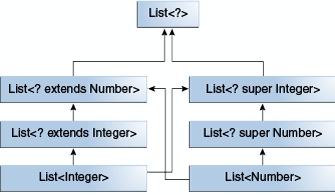
\includegraphics[height=4.5cm]{graph/generics-wildcardSubtyping}
    \end{figure}
\end{frame}
    
    \printbibliographyframe
    
	\section*{Kontakt}
	\begin{frame}{Kontakt}{}
	\begin{itemize}
		\item E-Mail: \href{mailto:lukas.abelt@airbus.com}{lukas.abelt@airbus.com}
		\item GitHub: \url{https://www.github.com/LuAbelt}
		\item GitLab: \url{https://www.gitlab.com/LuAbelt}
		\item Telefon(Firma): 07545 - 8 8895
		\item Telegram: LuAbelt
	\end{itemize}
\end{frame}
	

\end{document}